\chapter{System architecture}
\label{ch:architecture}

\lhead{Chapter 7. \emph{System architecture}}

\section{Overview}
\section{NIPEN}

\section{Front-end}

The main functionality of the front-end is to visualize the data stored by the Integration Platform.
This is accomplished by using a regular web-page consisting of HTML, CSS and JavaScript. HTML and CSS is used for structuring and giving a nice design of the web page. With help of JavaScript we are able to make the page dynamic.

\textbf{Design and Visualization}

One of the requirements given by the customer was that the front-end should use Helsenorge color palette. That is the front-end should use the colors shown in figure \ref{figure:helsenorge-color-palette}.

\begin{figure}[h]
\centering
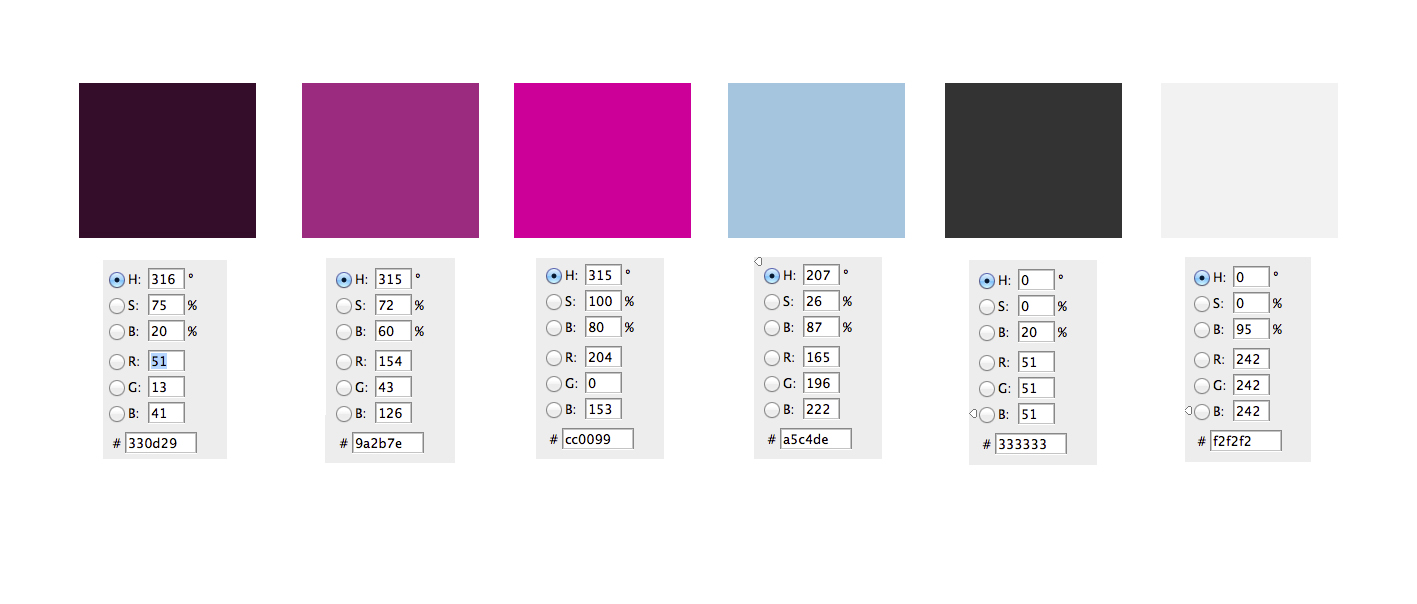
\includegraphics[scale=0.30]{../Figures/helsenorge_pallett.jpg}
\caption{Helsenorge color palette}
\label{figure:helsenorge-color-palette}
\end{figure}

\textbf{Retrieving the Data}

TODO

\textbf{Polling}

TODO

\section{Heart rate application}
\section{Weight application}
